\begin{frame}{Phương pháp trao đổi khóa}
Ý tưởng chung của các phương pháp trao đổi khóa như sau:
\begin{columns}
\column{0.4\textwidth}
\begin{figure}
    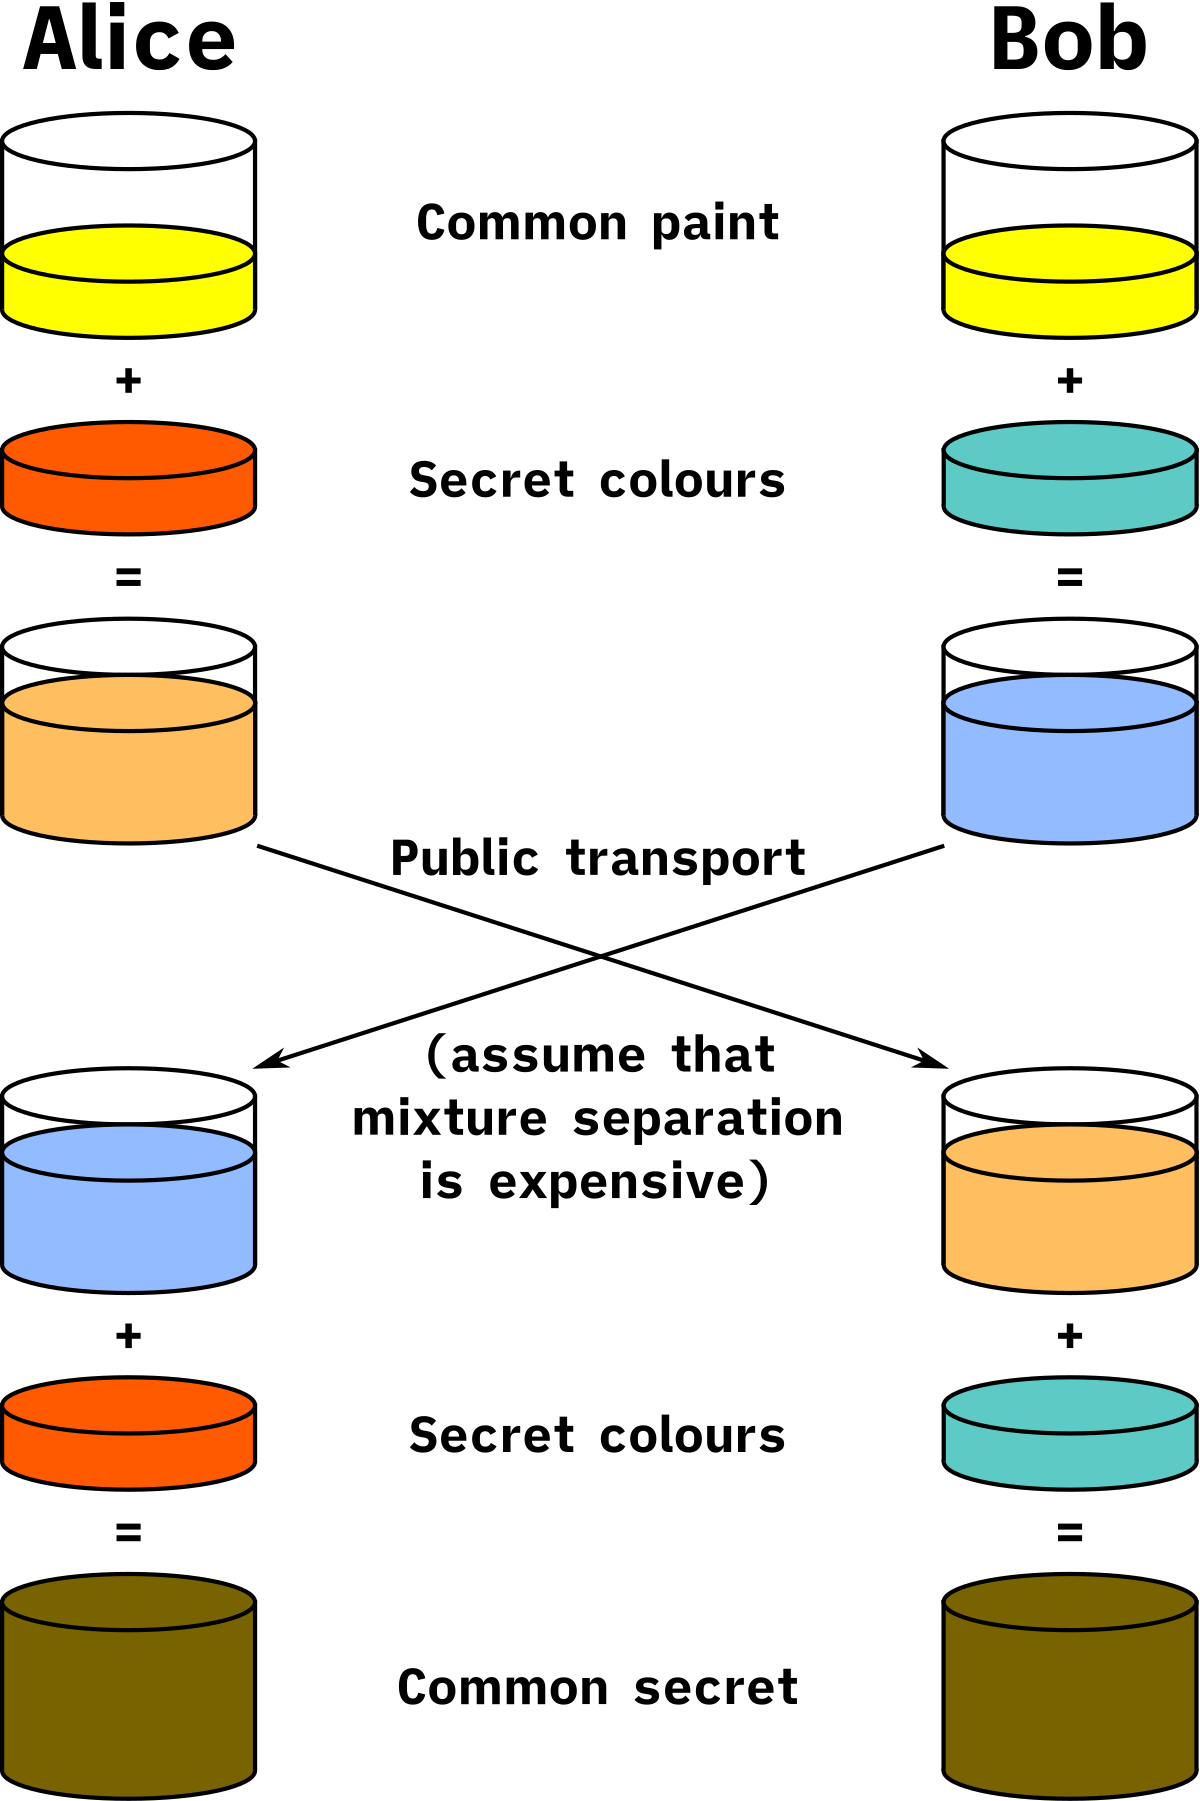
\includegraphics[scale=0.1]{diffie-hellman.png}
    \caption{Wikipedia}
\end{figure}

\column{0.6\textwidth}
\begin{enumerate}
    \item Alice và Bob thống nhất 1 khóa chung \textbf{G} (màu vàng)
    \item Alice chọn khóa bí mật \textbf{A} (màu đỏ) và Bob chọn khóa bí mật \textbf{B} (màu xanh)
    \item Alice tính khóa công khai của mình là \textbf{G+A} và gửi cho Bob. Bob tính khóa công khai của mình là \textbf{G+B} và gửi cho Alice
    \item Từ khóa công khai \textbf{G+B} của Bob, Alice tính được \textbf{G+B+A}
    \item Từ khóa công khai \textbf{G+A} của Alice, Bob tính được \textbf{G+A+B}
    \item Bây giờ Alice và Bob đều có \textbf{G+A+B} và sử dụng nó là khóa cho mã hóa đối xứng.
\end{enumerate}
\end{columns}
\end{frame}